\documentclass[aspectratio=169]{beamer}
\usepackage[utf8]{inputenc}
\usepackage{graphicx}
\usepackage{hyperref}
\usepackage{booktabs}
\usepackage{xcolor}
\usepackage{listings}
\usepackage[numbers]{natbib}       % numbered citations
\usepackage{attachfile2}
\usepackage{amsmath, amssymb}     % for align*, \mathcal, \text in math
\usepackage{tikz}

% Post-Mid badge helper
\newcommand{\postmidbadge}{%
  \begin{tikzpicture}[remember picture, overlay]
    \node[anchor=north east, xshift=-0.3cm, yshift=-0.1cm,
          fill=orange!20, draw=orange, rounded corners=3pt,
          font=\small\bfseries, text=orange!80!black, inner sep=4pt]
      at (current page.north east) {[Post-Mid]};
  \end{tikzpicture}%
}

\usetheme{Madrid}
\usecolortheme{default}

% Small gray citation command
\definecolor{darkgray}{RGB}{100,100,100}
\newcommand{\scite}[1]{{\footnotesize\color{darkgray}\citet{#1}}}

% Title – Final Evaluation
\title{Medical Diagnosis and Report Generation for Endoscopic Procedures Using Vision-Language Models}
\author{Praval Pattam, Theenesh Potluri, Pranav Sai Sarvepalli \\ \small Under the Guidance of: Dr.\ Jayaraj P B, Srinivasa T M \\ National Institute of Technology Calicut}
\date{B.Tech CSE Semester 8 Final Evaluation}

\setbeamertemplate{footline}[frame number]

\begin{document}

% ========== Title Slide ==========
\begin{frame}
\titlepage
\end{frame}

% ========== Agenda ==========
\begin{frame}{Agenda}
\tableofcontents
\end{frame}

% ========== Introduction Section ==========
\section{Introduction}

\begin{frame}
\centering \Large \textbf{Introduction}
\end{frame}

% --- The Clinical Burden ---
\begin{frame}{The Clinical Burden}
\begin{itemize}
    \item Each endoscopic procedure requires a \textbf{detailed written report} --- findings, diagnosis, and treatment recommendations
    \item Manual report writing takes \textbf{3--5 minutes per procedure}: a major bottleneck in high-volume GI units performing 30--50 cases per day
    \item A unit performing 40 procedures/day spends \textbf{$\sim$3.3 hours daily} on documentation alone --- time taken directly away from patient care
    \item Repetitive documentation contributes to \textbf{physician burnout} and diagnostic fatigue \scite{jama2024burden,bmj2024impact,nat2024burden}
    \item Documentation load has grown substantially with electronic health record requirements, doubling in the past decade \scite{nat2024burden}
\end{itemize}
\vspace{0.5em}
\textbf{Bottom line:} Time spent writing reports is time \textit{not} spent on patient care.
\end{frame}

% --- The AI Gap ---
\begin{frame}{The AI Gap}
\begin{itemize}
    \item General-purpose MLLMs (GPT-4V, LLaVA, Gemini) perform well on natural images but \textbf{fail on specialised endoscopy}:
    \begin{itemize}
        \item Cannot reliably identify subtle mucosal features (erythema, granularity, friability)
        \item Unfamiliar with endoscopic grading systems (Paris classification, Barrett's Prague criteria, ESGE grades)
        \item Produce generic descriptions rather than \textbf{structured clinical reports}
    \end{itemize}
    \item Existing medical MLLMs (LLaVA-Med, HuatuoGPT-Vision) are trained on broad biomedical data --- \textbf{not} on physician-annotated endoscopic reports
    \item \textbf{No model existed} trained on GMC Calicut physician-annotated GI endoscopic data, leaving a critical gap for Indian clinical settings
\end{itemize}
\end{frame}

% --- Our Objective ---
\begin{frame}{Our Objective}
\begin{block}{MVLMERG --- Multimodal Vision-Language Model for Endoscopic Report Generation}
Fine-tune a vision-language model to automatically generate professional-grade GI endoscopic reports.
\end{block}
\vspace{0.5em}
\begin{itemize}
    \item \textbf{Architecture:} LLaVA-4 base with CLIP-ViT-L/14 vision encoder + Vicuna-7B-v1.5 LLM backbone
    \item \textbf{Fine-tuning strategy:} P-LoRA --- soft prompt tuning + selective LoRA
    \item \textbf{Two-stage training:}
    \begin{enumerate}
        \item Stage 1: Medical domain knowledge injection (MedTrinity-25M,$\sim$160K Medical records)
        \item Stage 2: Physician-style report generation (GMC Calicut, $\sim$31,200 augmented samples)
    \end{enumerate}
    \item \textbf{Target:} Automated, structured, interpretable endoscopic reports in $\sim$\textbf{7 seconds} vs.\ 3--5 minutes manual
\end{itemize}
\end{frame}

% --- Problem Definition ---
\begin{frame}{Problem Definition}
\textbf{Core Problem:}
\begin{itemize}
    \item Writing endoscopic image reports requires deep domain expertise in gastroenterological terminology, lesion morphology, and clinical logic
    \item General Multimodal Large Language Models (MLLMs) exhibit critical knowledge gaps: they struggle with specialised endoscopy terminology, pathological feature descriptions, and complex medical reasoning
    \item Existing fine-tuning methods suffer from \textbf{limited domain adaptability} and \textbf{insufficient endoscopic-specific knowledge}
    \item High-quality physician-annotated endoscopic data is scarce --- publicly available medical datasets (PubMed) cover general medicine but lack the specificity needed for endoscopic report generation
\end{itemize}
\vspace{0.8em}
\textbf{Goal:} Develop \textbf{MVLMERG} --- a fine-tuned vision-language model that bridges the domain gap, producing professional-grade endoscopic reports matching the standard of intermediate-level physicians. \scite{pmc2024endo,frontiers2024survey}
\end{frame}

% --- Related Work: General Medical MLLMs ---
\begin{frame}{Related Work: General Medical MLLMs}
\begin{itemize}
    \item \textbf{LLaVA-Med} \scite{neurips2023llava} --- aligns PMC-15M biomedical image-text pairs in Stage 1; uses GPT-4-generated instruction data \scite{openai2023gpt4} for end-to-end fine-tuning in Stage 2; strong generalization but \textbf{lacks endoscopy-specific terminology}
    \item \textbf{HuatuoGPT-Vision} \scite{chen2024huatuo} --- refines medical image-text pairs from PubMed; MLLM-based denoising to build PubMedVision dataset; strong on broad medical VQA but \textbf{insufficient for detailed GI endoscopic findings}
    \item \textbf{BiomedGPT} \scite{zhang2024biomedgpt} --- unified generative pre-trained transformer across vision, language, and multimodal biomedical tasks; \textbf{broad coverage but weak on GI endoscopic report generation}
    \item \textbf{PeFoMed} \scite{frontiers2024survey} --- parameter-efficient fine-tuning framework for medical MLLMs; improves performance on medical imaging tasks but \textbf{not endoscopy-specific}
\end{itemize}
\vspace{0.3em}
\textbf{Common gap:} Broad biomedical pre-training cannot substitute for \textbf{physician-annotated, domain-specific} endoscopic training data.
\end{frame}

% --- Related Work: Surgical / GI-specific Models ---
\begin{frame}{Related Work: Surgical / GI-Specific Models}
\begin{itemize}
    \item \textbf{SurgicalGPT} --- fine-tuned GPT for surgical visual Q\&A; 3--5\% accuracy gain over generalist models but focuses on \textbf{surgical scenes}, not endoscopic mucosal analysis
    \item \textbf{ColonGPT / ColonINST} --- colonoscopy instruction tuning with polyp detection focus; good for classification but \textbf{not designed for full report generation}
    \item \textbf{EndoChat} --- endoscopy dialogue system; limited to conversational Q\&A format, \textbf{cannot produce structured clinical reports}
\end{itemize}
\vspace{0.8em}
\textbf{What all GI-specific models lack:}
\begin{itemize}
    \item None trained on \textbf{physician-annotated, full-format} endoscopic reports
    \item None target \textbf{Indian clinical settings} (terminology, grading conventions differ)
    \item None support complete structured report generation (findings + diagnosis + recommendations)
\end{itemize}
\end{frame}

% --- Related Work: Fine-Tuning Methods ---
\begin{frame}{Related Work: Fine-Tuning Methods}
\begin{itemize}
    \item \textbf{LoRA} \scite{lora2022hu} --- Low-Rank Adaptation; adds rank-decomposition matrices $\Delta W = BA$ to frozen weights; highly parameter-efficient but \textbf{no mechanism to align input representations} with the target domain
    \item \textbf{Prefix / P-Tuning} \scite{plora2022liu} --- soft prompt tokens prepended to input; aligns context but \textbf{without weight adaptation the model's knowledge remains unchanged}
    \item \textbf{PeFoMed} --- parameter-efficient fine-tuning for medical LLMs; effective for general medical Q\&A but \textbf{not evaluated on endoscopic scenarios}
    \item \textbf{MISS} --- parameter-efficient medical MLLM fine-tuning; covers multiple imaging modalities but \textbf{not endoscopy-specific}
\end{itemize}
\vspace{0.5em}
\textbf{Key insight:} Neither prompt tuning nor LoRA alone is sufficient --- their \textbf{combination (P-LoRA)} addresses both input representation alignment \textit{and} weight-space domain adaptation simultaneously.
\end{frame}

% --- Gap MVLMERG Fills ---
\begin{frame}{Gap MVLMERG Fills}
\begin{block}{The Gap}
No existing model combines (1) prompt-based input alignment, (2) selective weight adaptation, and (3) physician-annotated endoscopic training data.
\end{block}
\vspace{0.5em}
\begin{itemize}
    \item \textbf{P-LoRA} --- unifies soft prompt tuning + selective LoRA: addresses both input alignment and domain knowledge injection in a single fine-tuning strategy
    \item \textbf{GMC Calicut physician-annotated data} --- 6,500 real procedures annotated by senior endoscopists, augmented to $\sim$31,200 samples; reflects actual Indian clinical practice and terminology
    \item \textbf{Chain-of-Thought integration} --- anatomical $\to$ visual $\to$ diagnostic reasoning baked into training data; produces interpretable, verifiable reports
    \item \textbf{First model} targeting professional Indian GI endoscopic report generation in a real hospital deployment setting
\end{itemize}
\end{frame}

% ========== Methodology Section ==========
\section{Methodology}

\begin{frame}
\centering \Large \textbf{Methodology}
\end{frame}

% --- Dataset Creation and Augmentation ---
\begin{frame}{Dataset Creation and Augmentation}
\begin{itemize}
    \item \textbf{Data Source:} Government Medical College (GMC), Calicut
    \item \textbf{Raw Data:} 6,500 \textbf{patient reports} (semi‑structured PDFs + endoscopic images)
    \begin{itemize}
        \item Each report includes \textbf{4 endoscopic images}
    \end{itemize}
    \item \textbf{Data Augmentation:}
    \begin{itemize}
        \item Applied \textbf{rotation and random translation} to every image
        \item Purpose: increase dataset size and improve model robustness
        \item \textbf{Approximate scale:}
        \begin{itemize}
            \item Base Images = 9,000 (approx.)
            \item Rotation alone multiplies by 4 → over 36,000 images
            \item Translation variations further expand the pool
        \end{itemize}
    \end{itemize}
    \item \textbf{Text Data:}
    \begin{itemize}
        \item Final image--report pairs after augmentation: \textbf{$\sim$36,000 samples}
        \item Data split: 34,150 training / 1,850 validation
    \end{itemize}
    \item \textbf{Multimodal Association:} Each Q\&A pair linked to original + augmented endoscopic images \scite{arxiv2024qageneration,jmir2024instruction}
\end{itemize}
\end{frame}

% --- Figure 1: Custom Dataset Workflow ---
\begin{frame}{Figure 1: Custom Dataset Workflow}
\begin{figure}
\centering
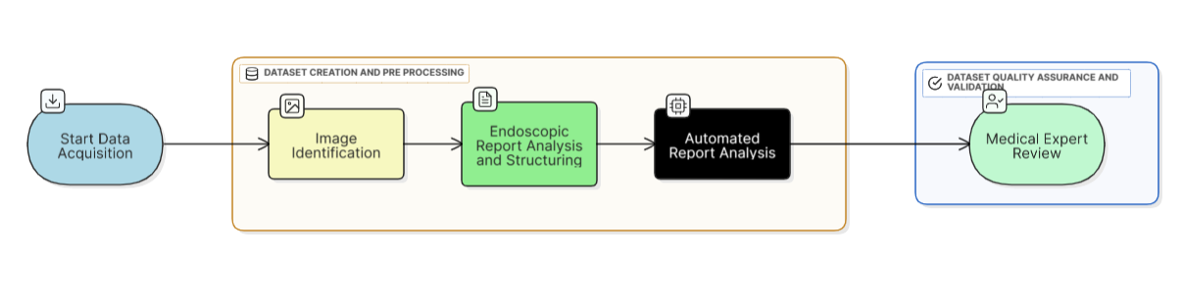
\includegraphics[width=0.9\textwidth]{figures/figure1_data_workflow.png}
\caption{Data Workflow: $\sim$36,000 image--report pair generation\scite{arxiv2024qageneration,jmir2024instruction}}
\end{figure}
\end{frame}

% --- Data Augmentation: Rotation ---
\begin{frame}{Data Augmentation: Rotation}
\postmidbadge
\begin{itemize}
    \item Each original endoscopic image is rotated by \textbf{0°, 90°, 180°, and 270°}
    \item Produces exactly \textbf{4 variants} per image
    \item Clinically safe: tissue textures and lesion appearances remain unchanged
    \item \textbf{Effect:} 4× structured expansion of the base image set
\end{itemize}
\end{frame}

% --- Data Augmentation: Stochastic Translation ---
\begin{frame}{Data Augmentation: Stochastic Translation}
\postmidbadge
\begin{itemize}
    \item \textbf{Sampling:} Bernoulli process with \( p=0.2 \) selects approx.\ 20\% of rotated images for translation
    \item \textbf{Shift model:} Translation vector \( (\tau_x,\tau_y) \) drawn from a truncated Gaussian:
    \begin{align*}
        \tau_x &\sim \mathcal{N}(0, (0.05\,W)^2),\; \text{clamped to } [-0.15\,W, +0.15\,W] \\
        \tau_y &\sim \mathcal{N}(0, (0.05\,H)^2),\; \text{clamped to } [-0.15\,H, +0.15\,H]
    \end{align*}
    \item \textbf{Overlap guarantee:}
    \[
        \text{Overlap Fraction} = \left(1 - \frac{|\tau_x|}{W}\right) \times \left(1 - \frac{|\tau_y|}{H}\right) \ge (1-0.15)^2 = 72.25\%
    \]
    \item \textbf{Result:} Controlled positional variation mimicking endoscopic camera jitter, without harming diagnostic content.
\end{itemize}
\end{frame}

% --- Data Augmentation Examples ---
\begin{frame}{Data Augmentation Examples}
\postmidbadge
\begin{figure}
\centering
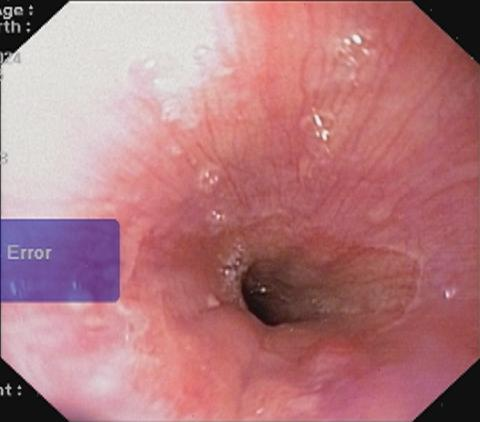
\includegraphics[height=4cm]{figures/aug_original.jpg}\hfill
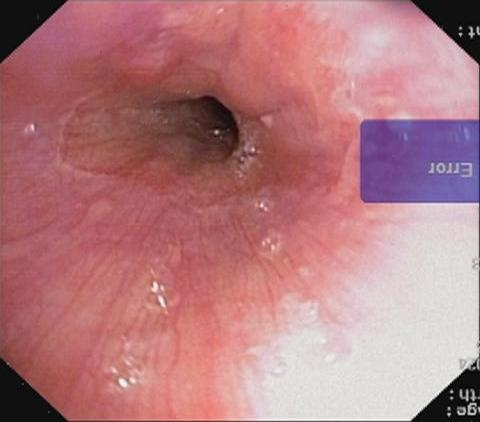
\includegraphics[height=4cm]{figures/aug_rotated_90.jpg}\hfill
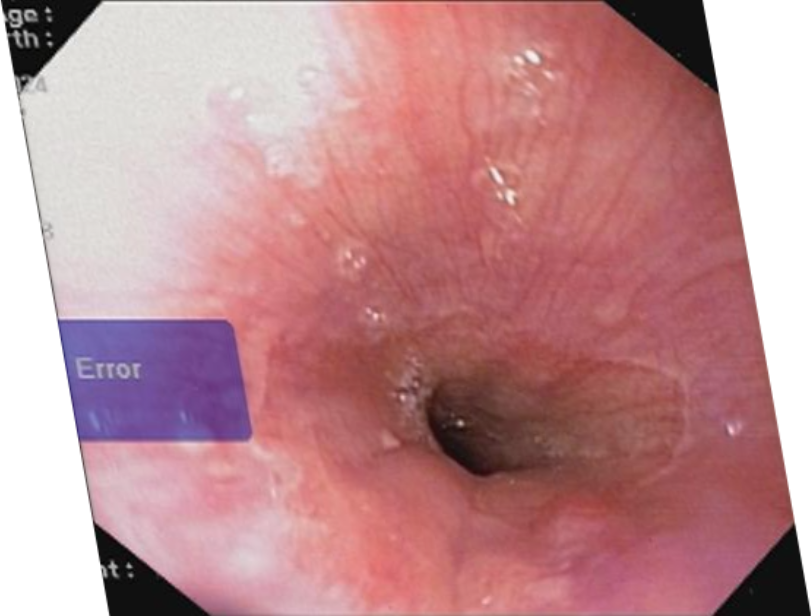
\includegraphics[height=4cm]{figures/aug_translated.png}
\caption{Left: Original \quad Middle: Rotated (90°) \quad Right: Randomly translated}
\end{figure}
\end{frame}

% --- Patient Data De-identification & Ethical Compliance ---
\begin{frame}{Patient Data De‑identification \& Ethical Compliance}
\begin{itemize}
    \item \textbf{Regulatory Framework \& Automated Script:}
    \begin{itemize}
        \item Strict adherence to the \textbf{Digital Personal Data Protection (DPDP) Act}, supported by a formal MoU between GMC Calicut and NIT Calicut
        \item \textbf{Redaction approach mirrors rigorous de‑identification used in recent high‑profile document releases} – all personally identifiable fields irreversibly blacked out to ensure zero traceability
        \item \textbf{Header Field Redaction:} Automatic blackout of Patient ID, Name, Age/Gender, Visit Date, UGI/OGD Numbers
    \end{itemize}
    \item \textbf{Result:} Irreversible anonymization of all sensitive patient information before data enters the pipeline
\end{itemize}
\vspace{0.5em}
\begin{figure}
\centering
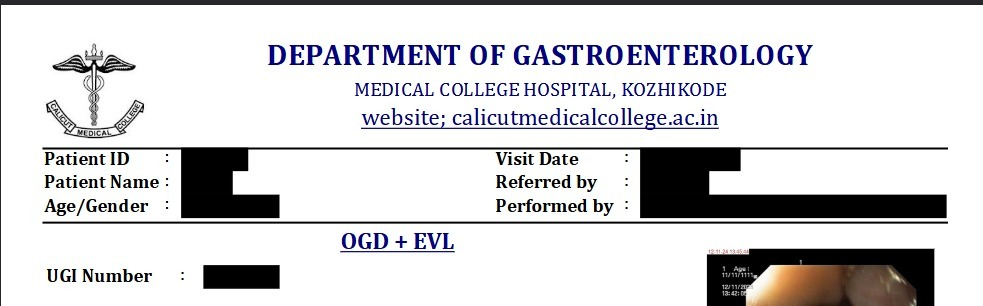
\includegraphics[width=0.85\textwidth, keepaspectratio]{figures/deidentification_diagram.jpeg}
\caption*{\textit{Irreversible de‑identification of sensitive info prior to the data pipeline.}}
\end{figure}
\end{frame}

% --- Report Analysis and Preprocessing (revised) ---
\begin{frame}{Report Analysis and Preprocessing}
\textbf{Medical Entities Extracted:} \scite{arxiv2024qageneration,jmir2024instruction}
\begin{itemize}
    \item Pathological findings and characteristics
    \item Diagnostic conclusions
    \item Procedural techniques and instruments
\end{itemize}
\vspace{1em}
\textbf{Processing Method:}
\begin{itemize}
    \item Natural language processing techniques
    \item Extraction of critical medical elements
    \item Foundation for Q\&A pair generation
\end{itemize}
\end{frame}

% --- Automated Question-Answer Pair Generation ---
\begin{frame}{Automated Question‑Answer Pair Generation}
\textbf{Multi‑Stage Process:} \scite{arxiv2024kvasir}
\begin{enumerate}
    \item \textbf{Medical Entity Extraction} – Key concepts and diagnoses
    \item \textbf{Question Template Design} – Diagnostic, anatomical, pathological, procedural, comparative
    \item \textbf{Automated QA Generation} -- Multiple question variations per concept \scite{neurips2023llava}
    \item \textbf{Answer Synthesis} – Accurate answers from reports + medical knowledge
\end{enumerate}
\vspace{1em}
\textbf{Result:} Diverse, clinically relevant question‑answer combinations.
\end{frame}

% --- GPT-5 Data Optimization & Filtering (slide 1: text) ---
\begin{frame}{Data Optimization \& Filtering with GPT-5}
\postmidbadge
\vspace{0.3em}
\textbf{Why GPT-5?} \scite{openai2023gpt4}
\begin{itemize}
    \item Physician reports from GMC Calicut contain incomplete, colloquial, or inconsistent sentences
    \item GPT-5 acts as an \textbf{auxiliary annotation tool} to enrich and templatize raw descriptions
    \item Structured prompt: \textit{``Convert to: This image shows (region). It describes (color, texture, features.)''}
    \item All GPT-5 outputs reviewed by senior gastroenterologists for clinical accuracy
\end{itemize}
\vspace{0.6em}
\textbf{Semantic Consistency Filter:} \scite{reimers2019sbert}
\begin{itemize}
    \item Optimized sentences must preserve the original clinical meaning
    \item Sentence-BERT extracts vector embeddings $\mathbf{u}$ (original) and $\mathbf{v}$ (enhanced)
    \item Cosine similarity: $S = \dfrac{\mathbf{u}\cdot\mathbf{v}}{\|\mathbf{u}\|\|\mathbf{v}\|}$ must satisfy $S > 0.85$
    \item If $S \leq 0.85$, GPT-5 regenerates until threshold is met
\end{itemize}
\end{frame}

% ========== Dataflow Pipeline and Methodology (2 image slides) ==========
\begin{frame}{Dataflow Pipeline and Methodology}
\begin{figure}
\centering
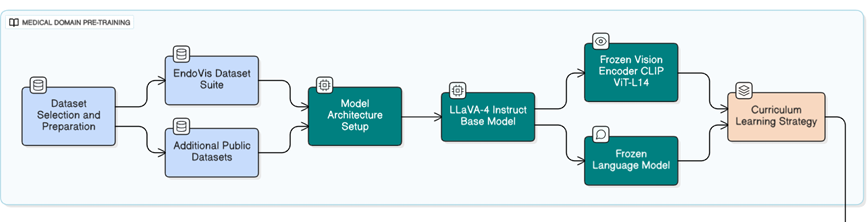
\includegraphics[width=\textwidth]{figures/pipeline_part1_data.png}
\caption{Stage 1: Pre-training.}
\end{figure}
\end{frame}

\begin{frame}{Dataflow Pipeline and Methodology}
\begin{figure}
\centering
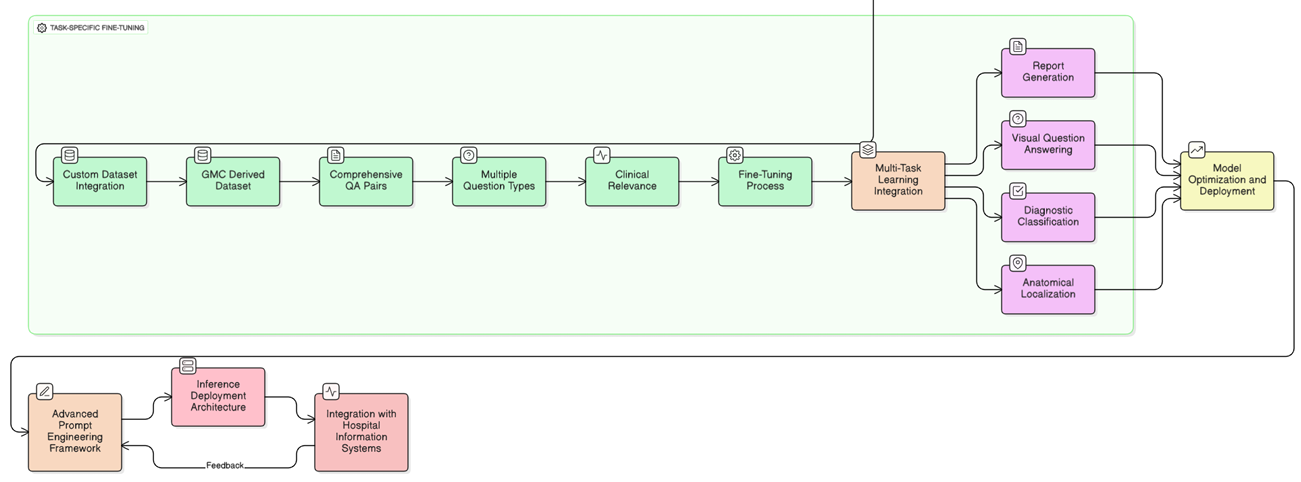
\includegraphics[width=\textwidth]{figures/pipeline_part2_training.png}
\caption{Stage 2: Fine-tuning}
\end{figure}
\end{frame}

% ========== Architecture Section ==========
\section{Architecture}

\begin{frame}
\centering \Large \textbf{Architecture}
\end{frame}

% --- Two‑Stage Training Framework (all original citations restored, now \scite) ---
\begin{frame}{Two‑Stage Training Framework --- MVLMERG}
    \textbf{Stage 1: Medical Domain Knowledge Injection} \scite{acl2024clinical,lora2022hu,zhang2026erglm}
\begin{itemize}
    \item \textbf{Objective:} Acquire gastrointestinal domain knowledge
    \item \textbf{Base Model:} LLaVA‑4 with frozen CLIP ViT‑L/14
    \item \textbf{Trainable:} LLM backbone (vision encoder + connector frozen)
    \item \textbf{Datasets:} MedTrinity-25M ($\sim$160K medical records) \scite{medtrinity2025xie,vqamed2019abacha}
\end{itemize}
\vspace{0.8em}
\textbf{Stage 2: Professional Report Generation} \scite{acl2024clinical,lora2022hu,zhang2026erglm}
\begin{itemize}
    \item \textbf{Objective:} Learn physician‑style endoscopic report language
    \item \textbf{Dataset:} GMC Calicut physician‑annotated data (6,500 base; $\sim$31K after augmentation)
        \item \textbf{Strategy:} P-LoRA --- prompt tokens + selective LoRA on key layers \scite{lora2022hu,plora2022liu,zhang2026erglm}
    \item \textbf{Unfrozen:} LLM backbone (vision encoder + connector frozen)
\end{itemize}
\end{frame}

% --- P-LoRA Overview ---
\begin{frame}{P-LoRA: Prompt-based LoRA Fine-Tuning}
\postmidbadge
P-LoRA combines \textbf{two complementary adaptation mechanisms}:

\vspace{0.3em}
\begin{columns}[T]
\begin{column}{0.48\textwidth}
\begin{block}{Soft Prompt Tuning \scite{plora2022liu,zhang2026erglm}}
Prepends $m = 64$ learnable tokens to the input embedding sequence --- steers the model's \textit{attention} toward endoscopic domain context before any weight computation.
\end{block}
\end{column}
\begin{column}{0.48\textwidth}
\begin{block}{Selective LoRA \scite{lora2022hu,zhang2026erglm}}
Injects low-rank adapter matrices $\Delta W = BA$ into the \textit{first, middle, and last} transformer layers --- adapts the model's \textit{knowledge} to endoscopic terminology and clinical report style.
\end{block}
\end{column}
\end{columns}
\vspace{0.5em}
\begin{itemize}
    \item Prompt tokens correct \textbf{input representation}; LoRA adapters correct \textbf{weight-space knowledge}
    \item Only \textbf{0.343\%} of all model parameters are trainable
\end{itemize}
\end{frame}

% --- Soft Prompt Tuning ---
\begin{frame}{Soft Prompt Tuning}
\vspace{0.2em}
\textbf{What it is:} \scite{plora2022liu}
\begin{itemize}
    \item $m = 64$ learnable embedding vectors $\{p_1, p_2, \ldots, p_{64}\}$ prepended to the input token sequence
    \item Updated via gradient descent during training --- \textbf{no manual prompt crafting required}
    \item At inference, the same learned tokens are prepended before every input
\end{itemize}
\vspace{0.5em}
\textbf{Why we use it:}
\begin{itemize}
    \item Manual prompts (e.g., ``You are a gastroenterologist\ldots'') are brittle and cannot encode fine-grained domain nuances
    \item Learnable tokens capture \textbf{implicit domain knowledge} --- endoscopic terminology, physician report style, grading conventions --- purely through the training signal
    \item The tokens guide the LLM's attention toward the clinical domain \textit{before} image and text tokens are processed
    \item Adds only $64 \times 4096 \approx 262$K parameters --- negligible overhead with significant domain alignment benefit
\end{itemize}
\end{frame}

% --- Selective LoRA ---
\begin{frame}{Selective LoRA}
\vspace{0.2em}
\textbf{What it is:} \scite{lora2022hu}
\begin{itemize}
    \item Low-rank adapter matrices injected into weight matrices: $W' = W + \Delta W = W + BA$
    \item $B \in \mathbb{R}^{d \times r}$, $A \in \mathbb{R}^{r \times k}$, rank $r = 64$, scaling $\alpha = 32$, dropout $= 0.05$
    \item Only $B$ and $A$ are trained; original $W$ is frozen
\end{itemize}
\vspace{0.4em}
\textbf{Why SELECTIVE (not all layers):}
\begin{itemize}
    \item Transformer layers \textbf{specialise} at different levels of abstraction:
    \begin{itemize}
        \item \textbf{Early layers} --- low-level syntax and token patterns; minimal domain shift needed
        \item \textbf{Middle layers} --- semantic composition and concept associations; \textbf{critical for medical terminology}
        \item \textbf{Last layers} --- task-specific output formatting and clinical report style
    \end{itemize}
    \item Targeting only these three groups \textbf{captures all domain adaptation needs} while training far fewer parameters
    \item Result: only \textbf{0.343\%} trainable parameters vs.\ $\sim$1\% for full LoRA --- same quality, faster training, lower GPU memory
\end{itemize}
\end{frame}

% --- Why P-LoRA beats LoRA alone ---
\begin{frame}{Why P-LoRA Outperforms LoRA Alone}
\vspace{0.2em}
\textbf{Plain LoRA --- the limitation:} \scite{lora2022hu,plora2022liu,zhang2026erglm}
\begin{itemize}
    \item Adapts weight matrices but does not change how the model \textit{interprets the input context}
    \item For highly specialised domains like GI endoscopy, the model still ``reads'' input through a generic lens --- producing suboptimal attention over clinical features
\end{itemize}
\vspace{0.4em}
\textbf{P-LoRA --- the combination advantage:}
\begin{itemize}
    \item \textbf{Prompt tokens} shift input representations toward the endoscopic domain \textit{before} attention is computed
    \item \textbf{LoRA adapters} then operate on already-domain-aligned representations --- more efficient weight updates with less training signal wasted
    \item The two mechanisms are \textbf{orthogonal}: prompt tuning acts at the input embedding level; LoRA acts at the weight matrix level
\end{itemize}
\vspace{0.4em}
\textbf{Empirical gains over plain LoRA:}
\begin{itemize}
    \item \textbf{+5\% CIDEr} and \textbf{+4.4\% ROUGE-L} over plain LoRA
    \item GPU memory: $\sim$43 GB (comparable to plain LoRA $\sim$44 GB)
    \item Inference: $\sim$7 s/report
\end{itemize}
\end{frame}

% --- System Architecture Diagram ---
\begin{frame}{System Architecture}
\begin{figure}
\centering
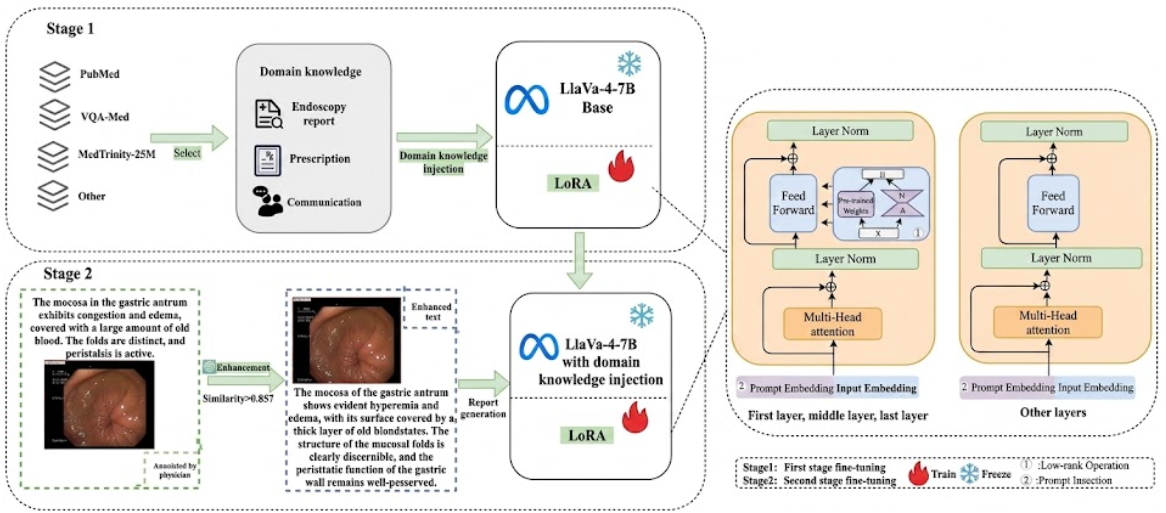
\includegraphics[width=\textwidth]{figures/system_architecture.png}
\caption{High‑level architecture of the proposed vision‑language model for endoscopic report generation.}
\end{figure}
\end{frame}

% --- Model Architecture – LLaVA ---
\begin{frame}{Model Architecture – LLaVA}
\begin{figure}
\centering
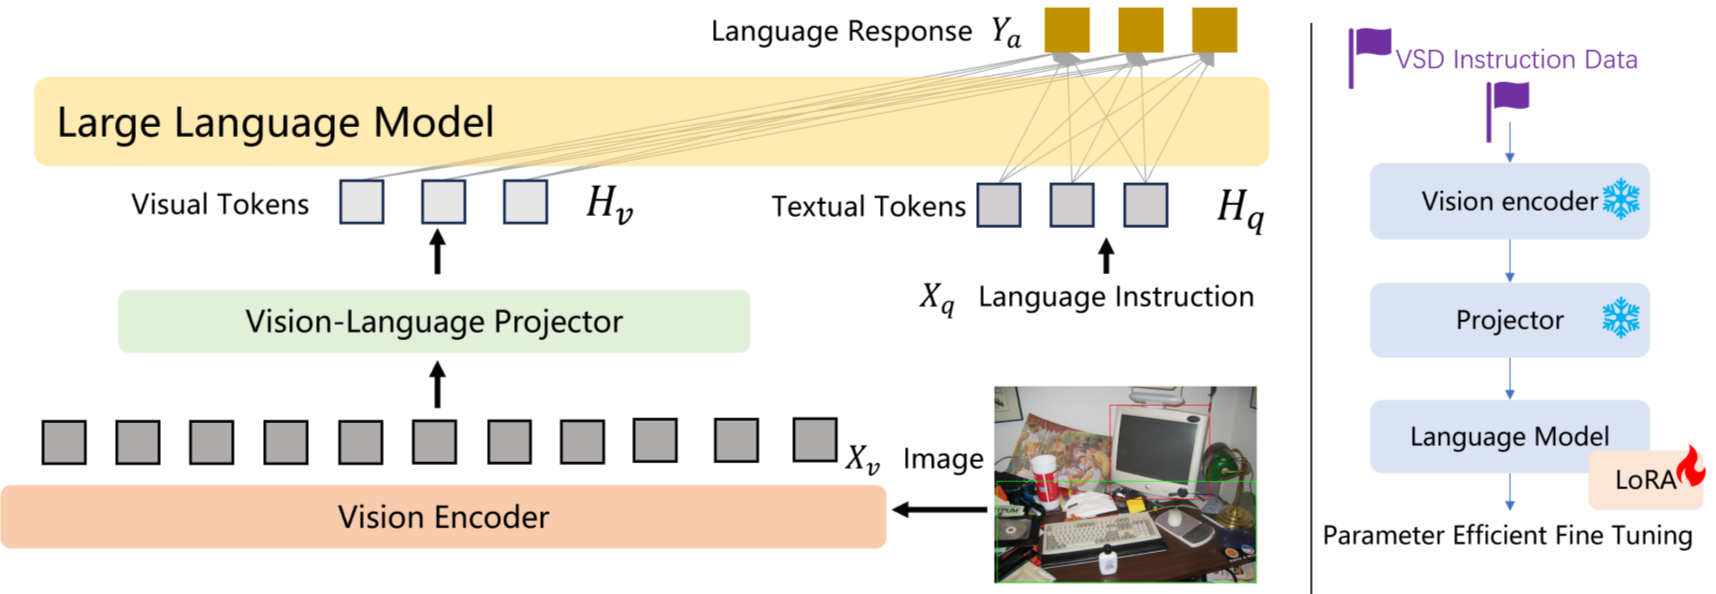
\includegraphics[width=\textwidth]{figures/llava_architecture.png}
\caption{LLaVA architecture: vision encoder + projection layer + language model for multimodal understanding.}
\end{figure}
\end{frame}

% --- CLIP‑ViT Architecture ---
\begin{frame}{CLIP‑ViT Architecture}
\begin{figure}
\centering
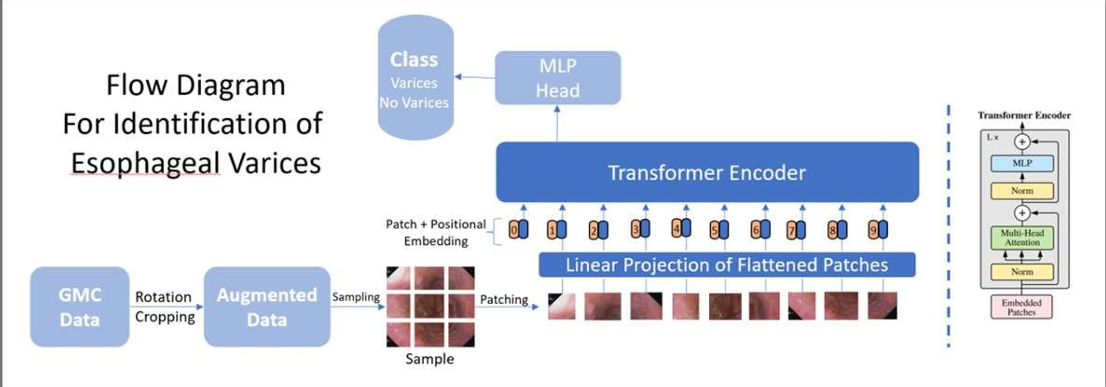
\includegraphics[width=\textwidth]{figures/clip_vit_architecture.png}
\caption{CLIP‑ViT‑L/14 vision encoder: patch embedding, transformer layers, and projected visual features.}
\end{figure}
\end{frame}

% --- Vicuna Architecture ---
\begin{frame}{LLM Backbone --- Vicuna-7B-v1.5}
\begin{figure}
\centering
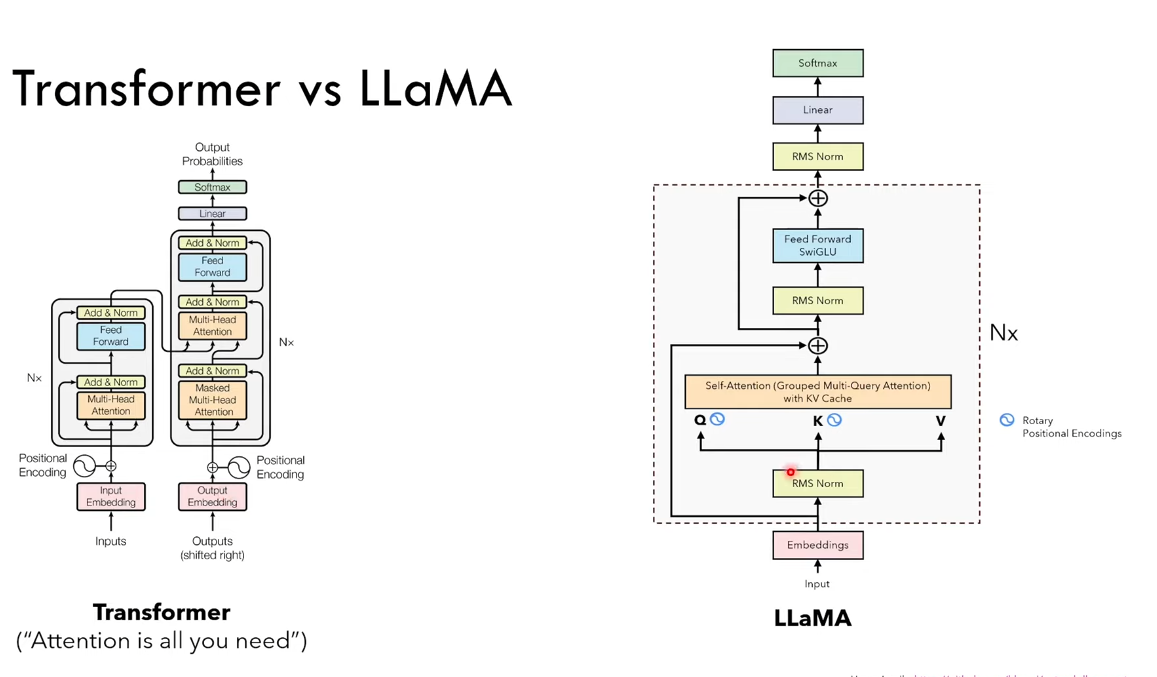
\includegraphics[width=\textwidth]{figures/llama_architecture.png}
\caption{Vicuna-7B-v1.5 language model backbone (based on LLaMA decoder architecture): transformer decoder layers used for text generation and multimodal fusion.}
\end{figure}
\end{frame}

% ========== Implementation Section ==========
\section{Implementation}

\begin{frame}
\centering \Large \textbf{Implementation}
\end{frame}

% --- Refining Generation: Implementing System Prompts ---
\begin{frame}{Refining Generation: Implementing System Prompts}
\textbf{Initial Challenge:} 
\begin{itemize}
    \item Early model iterations produced verbose, unstructured, and redundant reports that did not match standard clinical formatting.
\end{itemize}

\vspace{0.8em}
\textbf{Implemented Solution (Dataset Reformatting):}
\begin{itemize}
    \item Integrated rigorous \textbf{System Prompts} directly into the training dataset.
    \item \textbf{Role Assignment:} Instructed the model to assume a specific clinical persona (e.g., ``You are an expert gastroenterologist...'').
    \item \textbf{Output Constraints:} Provided explicit instructions to prioritise direct, concise, and structured answers mirroring real GMC Calicut reports.
\end{itemize}

\vspace{0.5em}
\textbf{Result:} A massive reduction in unnecessary text, yielding highly concise and structured outputs; further refinement improved diagnostic accuracy.
\end{frame}

% --- Qualitative Impact: Verbose vs. Concise Reports (unchanged) ---
\begin{frame}{Qualitative Impact: Verbose vs. Concise Reports}
\begin{columns}[T]
    \begin{column}{0.48\textwidth}
        \centering
        \textbf{\textcolor{red}{Previous Generation}} \\
        \textit{(Verbose \& Redundant)}
        \vspace{0.5em}
        \only<1>{\fbox{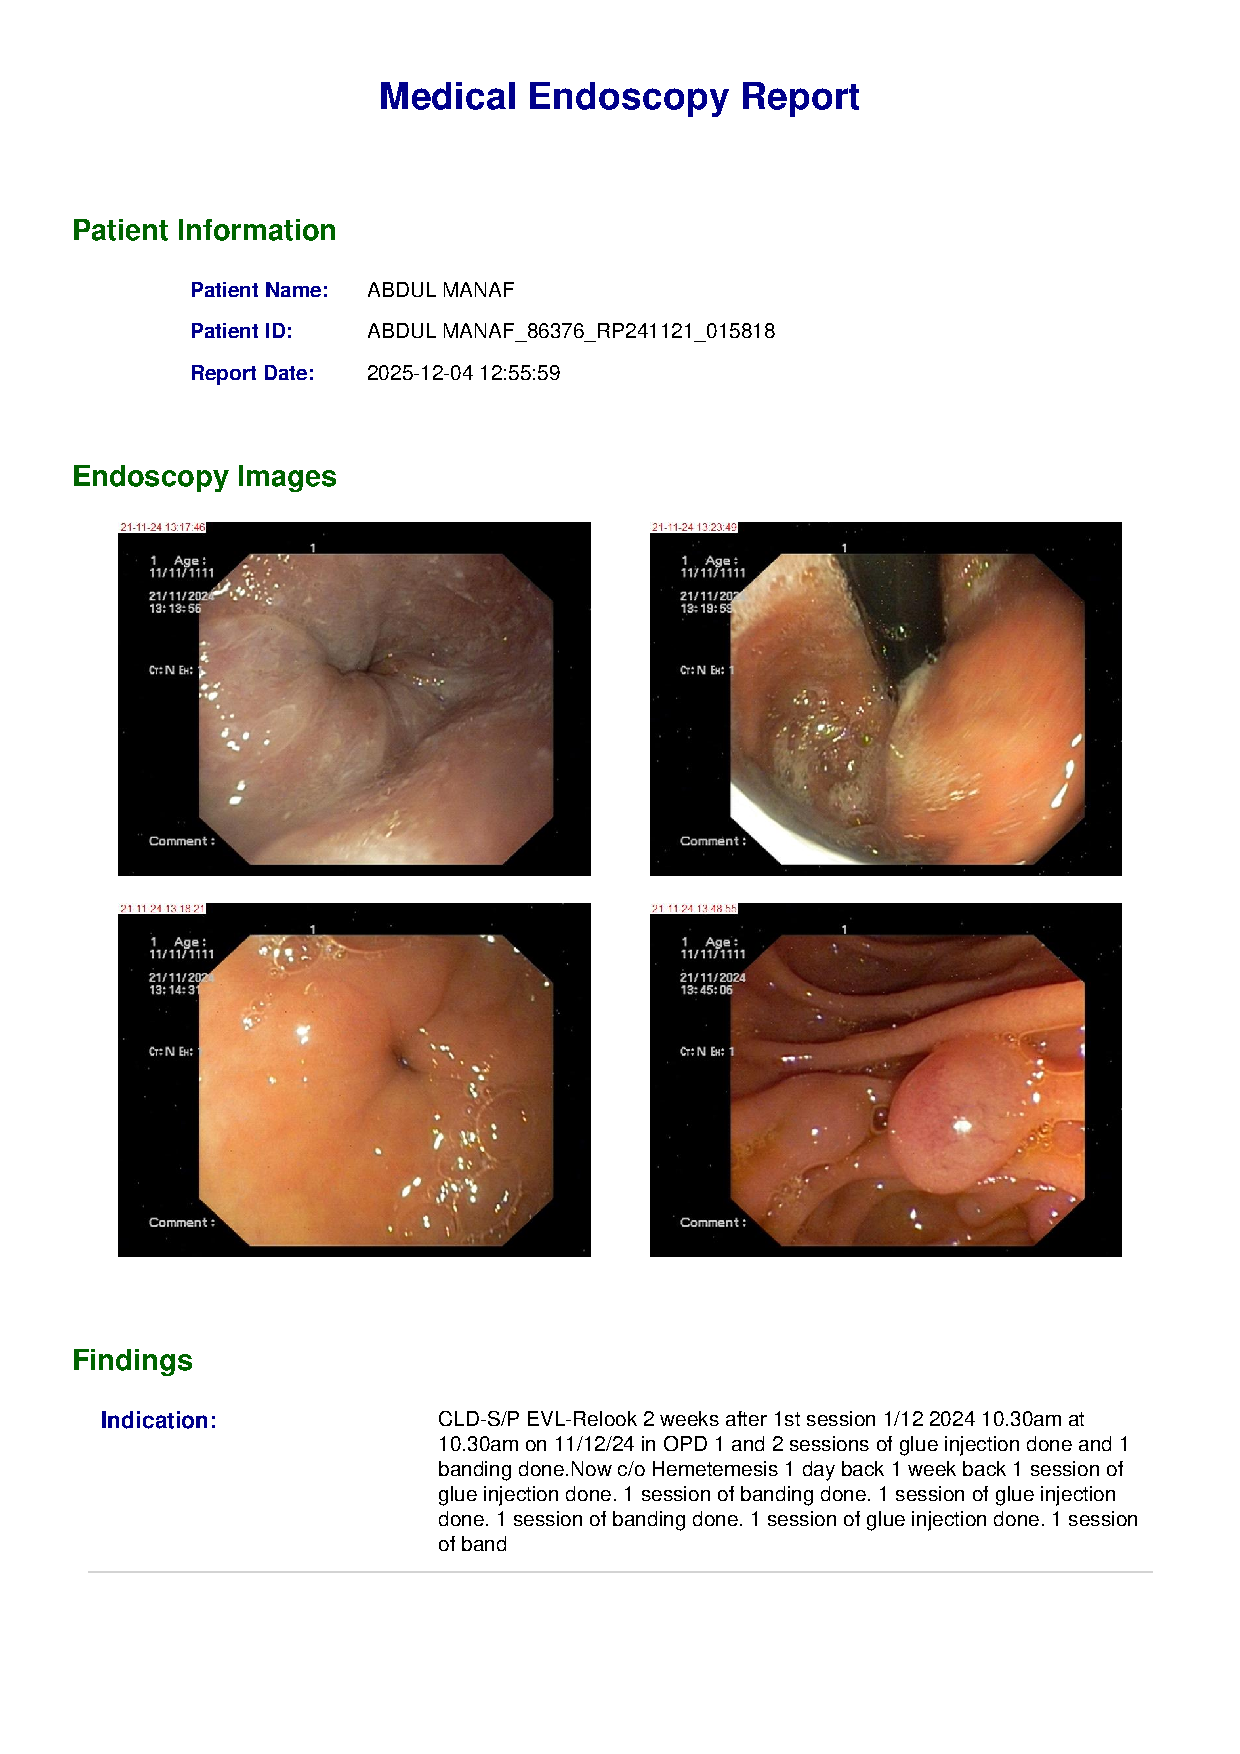
\includegraphics[page=1, trim=1cm 3cm 1cm 1cm, clip, width=\textwidth]{figures/old_report.pdf}}}
        \only<2>{\fbox{\includegraphics[page=2, trim=1cm 3cm 1cm 1cm, clip, width=\textwidth]{figures/old_report.pdf}}}
    \end{column}
    \begin{column}{0.48\textwidth}
        \centering
        \textbf{\textcolor{blue}{Current Generation}} \\
        \textit{(Concise via System Prompt)}
        \vspace{0.5em}
        \only<1>{\fbox{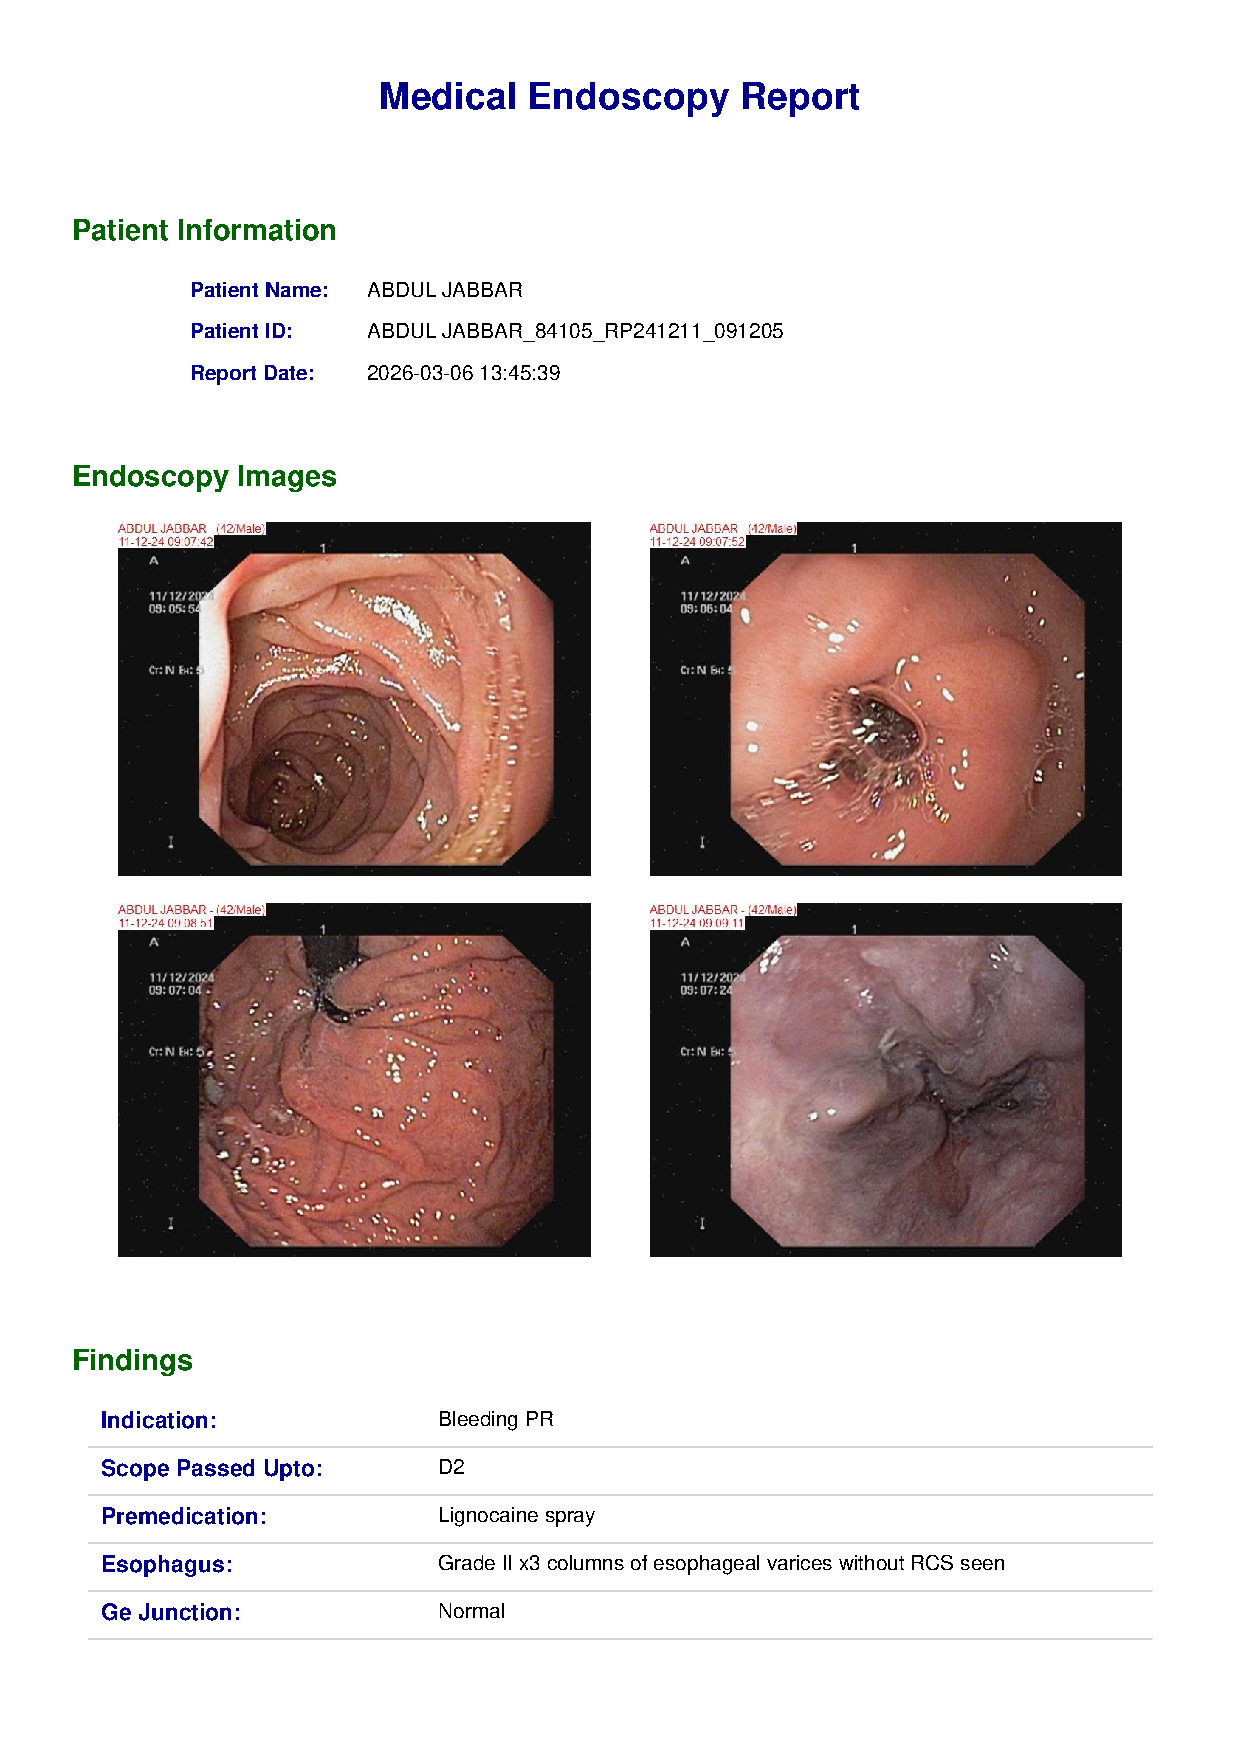
\includegraphics[page=1, trim=1cm 10cm 1cm 1cm, clip, width=\textwidth]{figures/new_report.pdf}}}
        \only<2>{\fbox{\includegraphics[page=2, trim=1cm 10cm 1cm 1cm, clip, width=\textwidth]{figures/new_report.pdf}}}
    \end{column}
\end{columns}
\vspace{0.5em}
\centering
\textbf{\only<1>{Page 1 Comparison}\only<2>{Page 2 Comparison}}
\end{frame}

% --- The “Blackbox” Problem & Our Solution ---
\begin{frame}{The “Blackbox” Problem \& Our Solution}
\textbf{The Initial Blackbox:}
\begin{itemize}
    \item The model would output a final diagnosis directly from an image without revealing its reasoning, making it hard to trust or debug.
\end{itemize}

\vspace{0.8em}
\textbf{Our Solution – Chain‑of‑Thought Integration:}
\begin{itemize}
    \item Augmented the training Q\&A pairs with \textbf{step‑by‑step reasoning chains}.
    \item Each chain forces the model to structure its answer as: \textbf{anatomical identification → visual observation → diagnosis}.
    \item During training, the model learns to mimic this transparent reasoning process.
\end{itemize}

\vspace{0.5em}
\textbf{Outcome:} The model now explicitly explains \textit{what it sees} and \textit{why it concludes something}, turning a black‑box predictor into an \textbf{interpretable diagnostic assistant}.
\end{frame}

% --- Chain‑of‑Thought (CoT) in Endoscopy (now implemented) ---
\begin{frame}{Chain‑of‑Thought (CoT) in Endoscopy}
\postmidbadge
\textbf{Before CoT Implementation (Baseline Model):}
\begin{itemize}
    \item \textbf{Input:} [Image] ``What is the diagnosis?''
    \item \textbf{Output:} ``Grade II Esophageal Varices.'' \textit{(correct but no justification)}
\end{itemize}

\vspace{1em}
\textbf{After CoT Implementation (Our Model):}
\begin{itemize}
    \item \textbf{Input:} [Image] ``Analyze the image step‑by‑step and provide a diagnosis.''
    \item \textbf{Output:} 
    \begin{enumerate}
        \item \textbf{Observation 1:} I observe the lower third of the oesophagus.
        \item \textbf{Observation 2:} There are swollen, tortuous submucosal veins present.
        \item \textbf{Observation 3:} The veins occupy less than 1/3 of the lumen, with no red colour signs.
        \item \textbf{Conclusion:} Therefore, the diagnosis is Grade II Esophageal Varices.
    \end{enumerate}
\end{itemize}
\vspace{0.5em}
\textbf{Impact:} Explicit reasoning enhances clinical trust, allows verification, and helps identify subtle mistakes – a crucial feature for real‑world deployment.
\end{frame}

% --- Fine‑Tuning Configuration Details ---
\begin{frame}{Fine‑Tuning Configuration Details}
\textbf{Vision Encoder:} CLIP‑ViT‑L/14
\begin{itemize}
    \item Image resolution: 336×336 pixels
    \item Patch size: 14×14 (24×24 grid)
    \item Total vision tokens: 577 per image (576 patches + CLS)
\end{itemize}

\vspace{0.8em}
\textbf{Training Hyperparameters:}
\begin{itemize}
    \item \textbf{Precision:} bfloat16 (BF16)
    \item \textbf{Optimizer:} AdamW with 8‑bit quantization
    \item \textbf{Learning Rate:} 2e$^{-4}$ with cosine scheduler, warmup 0.1
    \item \textbf{Batch Size:} 2 micro‑batch, 4 accumulation steps = 8 global
    \item \textbf{Attention:} Flash Attention 2
    \item \textbf{Epochs:} 4 epochs (both stages)
\end{itemize}
\end{frame}

% --- Training Configuration Rationale ---
\begin{frame}{Training Configuration Rationale}
\begin{itemize}
    \item \textbf{CLIP‑ViT‑L/14} – pre‑trained on 400M pairs; robust medical visual features; L size balances capacity vs. speed; 14×14 patch grid captures both anatomy and small lesions.
    \item \textbf{336×336 resolution} – standard for LLaVA; sufficient detail without excessive memory.
    \item \textbf{577 vision tokens} – each patch token carries localised information, enabling the language model to ``see'' global and local structures.
    \item \textbf{bfloat16} – halves memory vs. FP32, no performance loss.
    \item \textbf{AdamW + 8‑bit} – stable weight‑decoupled convergence; 8‑bit reduces optimizer memory ~75\%.
    \item \textbf{LR 2e$^{-4}$, cosine + warmup} – low peak prevents catastrophic forgetting; warmup stabilises early steps.
    \item \textbf{Batch size 8 (accumulated)} – simulates larger batch under GPU memory limits.
    \item \textbf{Flash Attention 2} – memory‑efficient exact attention; ~5‑10× VRAM reduction for long sequences.
    \item \textbf{4 epochs} – sufficient for P-LoRA adapters on the augmented second-stage dataset without overfitting.
\end{itemize}
\end{frame}

% --- Why AdamW & Flash Attention 2? (concise) ---
\begin{frame}{Why AdamW \& Flash Attention 2?}
\textbf{AdamW over Adam}
\begin{itemize}
    \item Adam couples weight decay with gradient scaling – can over‑regularize.
    \item AdamW \textbf{decouples} weight decay from adaptive gradients → better generalization.
    \item Standard for LLaMA fine‑tuning; prevents over‑shrinking of LoRA adapters.
\end{itemize}
\vspace{0.5em}
\textbf{Flash Attention 2 over regular / Flash Attention 1}
\begin{itemize}
    \item Standard attention: O(N$^2$) memory – prohibitive for 577 vision tokens + text.
    \item Flash Attention 1 tiled computation, but under‑utilised GPU parallelism.
    \item Flash Attention 2:
    \begin{itemize}
        \item \textbf{Fewer non‑matmul operations} → higher throughput.
        \item \textbf{Better batch/head parallelism} → faster training.
        \item \textbf{Lower VRAM usage (5‑10× reduction)} → feasible on single GPU.
    \end{itemize}
\end{itemize}
\vspace{0.5em}
\textbf{Together:} Stable convergence + memory‑efficient training at scale.
\end{frame}

% ========== Results Section ==========
\section{Results}

\begin{frame}
\centering \Large \textbf{Results}
\end{frame}


% --- Generated Report – Two Pages Side by Side ---
\begin{frame}{Generated Report}
\begin{columns}[T]
    \begin{column}{0.48\textwidth}
        \centering
        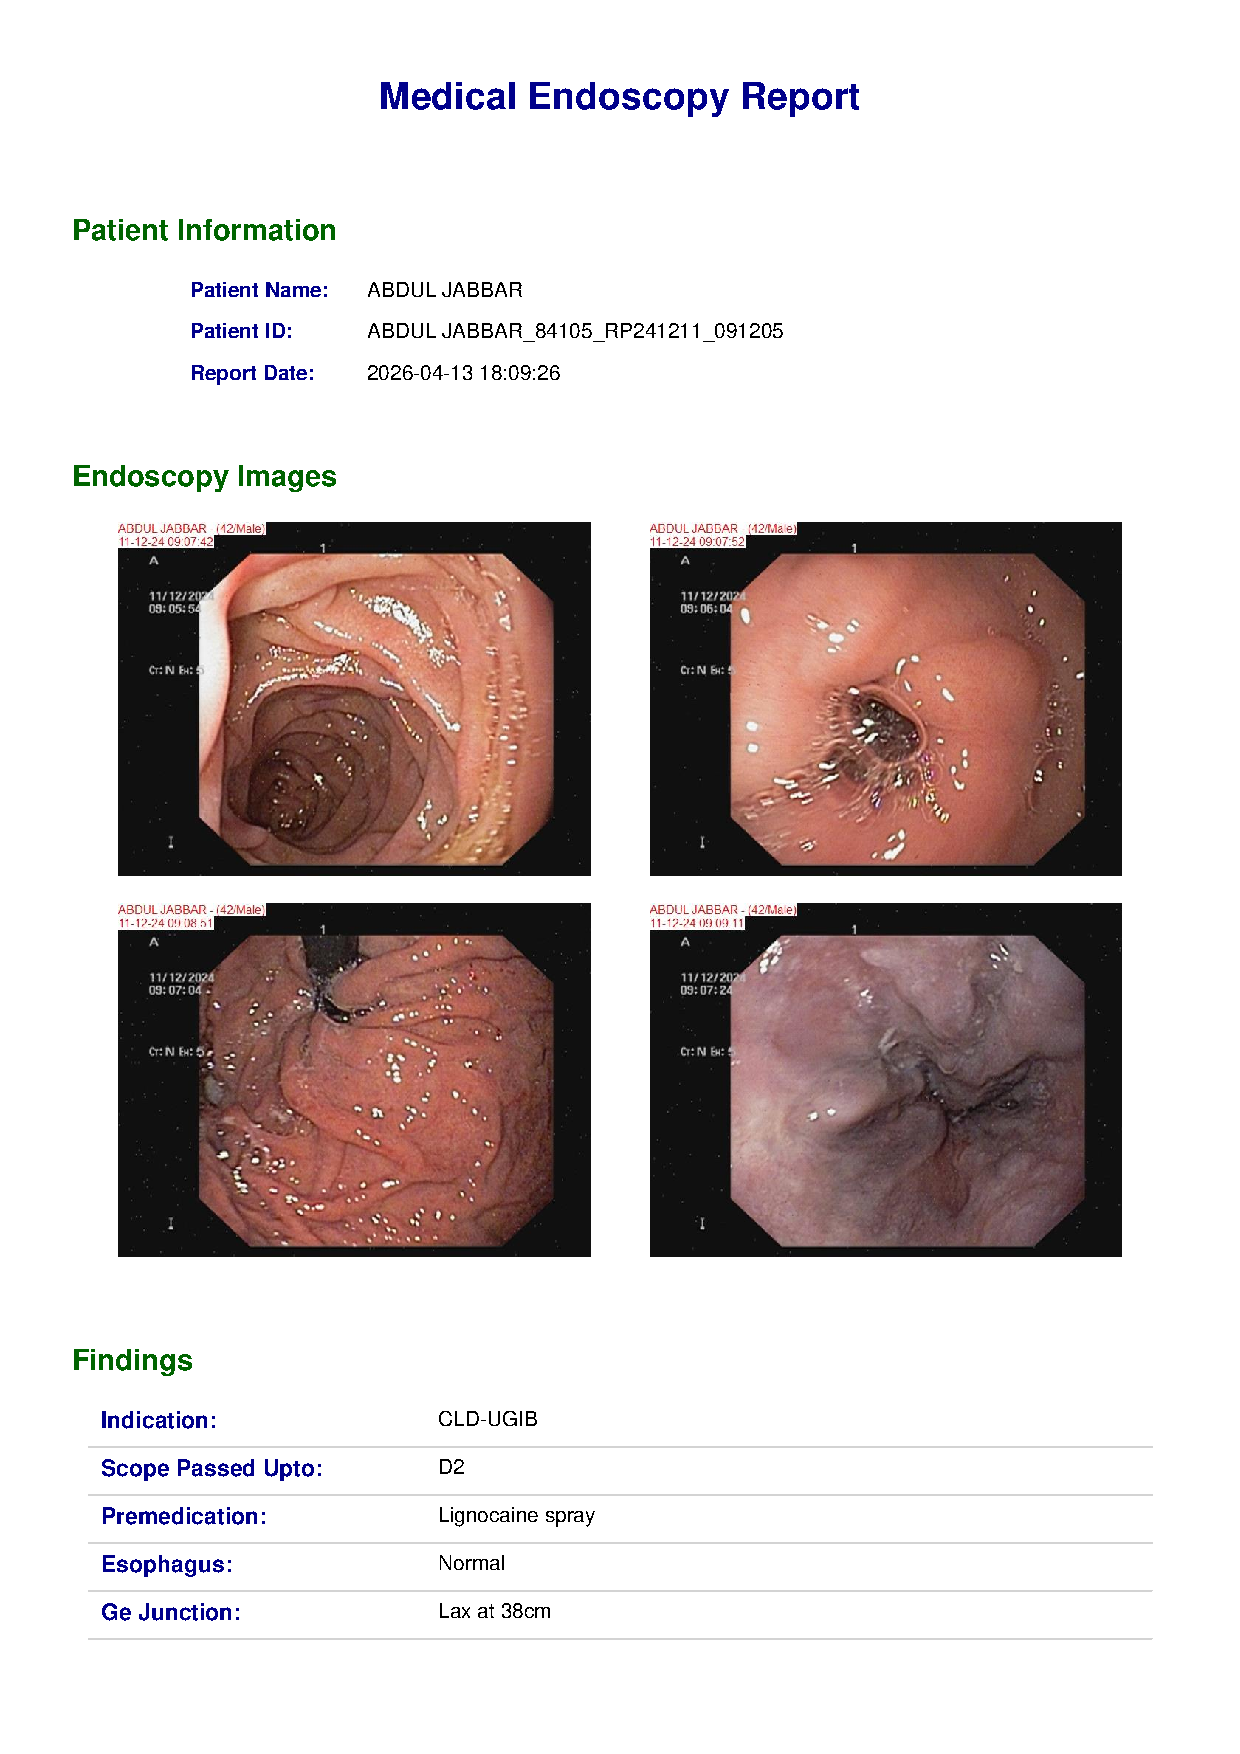
\includegraphics[height=0.82\textheight, keepaspectratio, page=1]{generated_report.pdf}
    \end{column}
    \begin{column}{0.48\textwidth}
        \centering
        \includegraphics[height=0.82\textheight, keepaspectratio, page=2]{generated_report.pdf}
    \end{column}
\end{columns}
\vspace{0.3em}
\centering
\small Final diagnostic report – Pages 1 and 2
\end{frame}


% --- Evaluation Metrics Slide 1: Formulas ---
\begin{frame}{Evaluation Metrics}
\begin{columns}[T]
\column{0.48\textwidth}

\small
\textbf{CIDEr} \\
Consensus-based evaluation using TF-IDF weighted n-gram vectors.
{\footnotesize
\[\text{CIDEr}(c,S)=\frac{1}{M}\sum_{m}\frac{\mathbf{g}^n(c)\cdot\mathbf{g}^n(s_m)}{\|\mathbf{g}^n(c)\|\,\|\mathbf{g}^n(s_m)\|}\]}

\vspace{0.2cm}
\textbf{ROUGE-L} \\
F-measure based on longest common subsequence (LCS).
{\footnotesize
\[\text{ROUGE-L}=\frac{(1+\beta^2)\,R_{lcs}\cdot P_{lcs}}{R_{lcs}+\beta^2 P_{lcs}}\]}

\vspace{0.2cm}
\textbf{METEOR} \\
Combines precision, recall, and a fragmentation penalty.
{\footnotesize
\[F_{mean}=\frac{10 P R}{R+9P},\quad\text{METEOR}=F_{mean}(1-\text{Pen})\]}

\column{0.48\textwidth}

\small
\textbf{BLEU-4} \\
Geometric mean of 1--4 gram precisions with brevity penalty.
{\footnotesize
\[\text{BLEU-4}=\text{BP}\cdot\exp\!\left(\frac{1}{4}\sum_{n=1}^{4}\log p_n\right)\]}

\vspace{0.2cm}
\textbf{BERTScore} \\
Semantic similarity via contextual BERT token embeddings.
{\footnotesize
\[F_{\text{BERT}}=\frac{2\,P_{\text{BERT}}\cdot R_{\text{BERT}}}{P_{\text{BERT}}+R_{\text{BERT}}}\]}

\vspace{0.4cm}
\small All five metrics reward similarity to reference reports; higher is better ($\uparrow$).
\end{columns}
\end{frame}

% --- Evaluation Metrics Slide 2: Why these metrics? ---
\begin{frame}{Why These Evaluation Metrics?}
\begin{columns}[T]
\begin{column}{0.48\textwidth}
\small\textbf{CIDEr} --- \textit{primary metric}
\begin{itemize}\setlength\itemsep{0pt}
    \item Designed for report generation; TF-IDF up-weights \textit{discriminative} n-grams, penalising generic filler
    \item Best reflects domain-specific clinical term quality
\end{itemize}
\textbf{ROUGE-L} --- \textit{clinical structure}
\begin{itemize}\setlength\itemsep{0pt}
    \item LCS-based: captures correct finding sequence (anatomy $\to$ observation $\to$ diagnosis)
    \item Robust to paraphrasing
\end{itemize}
\textbf{METEOR} --- \textit{linguistic fluency}
\begin{itemize}\setlength\itemsep{0pt}
    \item Handles synonyms and stemming --- physicians use varied clinical vocabulary
    \item Fragmentation penalty discourages incoherent output
\end{itemize}
\end{column}
\begin{column}{0.48\textwidth}
\small\textbf{BLEU-4} --- \textit{n-gram precision}
\begin{itemize}\setlength\itemsep{0pt}
    \item 4-gram precision captures multi-word phrases (e.g., ``Grade II esophageal varices'')
    \item Included for comparability with prior medical NLG literature
\end{itemize}
\textbf{BERTScore} --- \textit{semantic correctness}
\begin{itemize}\setlength\itemsep{0pt}
    \item Contextual BERT embeddings measure semantic similarity beyond surface overlap
    \item Handles spelling variants (``oesophageal'' vs.\ ``esophageal'')
    \item Strongest indicator of correct clinical meaning
\end{itemize}
\end{column}
\end{columns}
\end{frame}

% --- Quantitative Comparison ---
\begin{frame}{Quantitative Comparison --- MVLMERG vs. Baselines}
\centering
\resizebox{\textwidth}{!}{%
\begin{tabular}{lccccc}
\toprule
\textbf{Method} & \textbf{CIDEr}$\uparrow$ & \textbf{ROUGE-L}$\uparrow$ & \textbf{METEOR}$\uparrow$ & \textbf{BLEU-4}$\uparrow$ & \textbf{BERTScore}$\uparrow$ \\
\midrule
Qwen2-VL-7B-Instruct & 0.0078 & 0.0504 & 0.0564 & 0.0009 & 0.8317 \\
BLIP-2    & 0.0079 & 0.0147 & 0.0347 & 0.0002 & 0.7957 \\
InstructBLIP & 0.0088 & 0.0320 & 0.0583 & 0.0004 & 0.8196 \\
\textbf{Our Model}   & \textbf{0.0531} & \textbf{0.2632} & \textbf{0.1187} & \textbf{0.0006} & \textbf{0.8760} \\
\bottomrule
\end{tabular}%
}
\vspace{0.4em}
\small Evaluated on 100 samples. MVLMERG leads on 4 of 5 metrics (CIDEr, ROUGE-L, METEOR, BERTScore). \\
\footnotesize\textit{Note: BLEU-4 (0.0006) is marginally below Qwen2-VL (0.0009); all other metrics show clear improvement.}
\end{frame}

% --- Expert Physician Evaluation ---
\begin{frame}{Expert Physician Evaluation}
\vspace{0.3em}
\textbf{Evaluation Protocol:} \scite{pmc2024endo}
\begin{itemize}
    \item 2 senior endoscopists (10+ years experience), GMC Calicut
    \item Each generated report labelled \textbf{Correct / Incorrect} based on clinical accuracy
    \item Disagreements resolved by \textbf{joint review and consensus discussion}
\end{itemize}
\vspace{0.3em}

\end{frame}

% --- Hardware \& Training Setup ---
\begin{frame}{Hardware \& Training Setup}
\begin{columns}[T]
\begin{column}{0.5\textwidth}
\textbf{Training Hardware:}
\begin{itemize}
    \item \textbf{GPU:} NVIDIA H200 NVL 143 GB HBM3e (CUDA 13.0)
    \item \textbf{CPU:} Intel Xeon 6505P\\(12 cores/socket, 2 sockets, 48 threads)
    \item \textbf{RAM:} 251 GiB
    \item \textbf{Python:} 3.12.3; PyTorch 2.11.0+cu130 (BF16 + Flash Attention 2)
\end{itemize}
\vspace{0.5em}
\textbf{Training Resource Usage:}
\begin{itemize}
    \item GPU memory during training: $\sim$43 GB
    \item Trainable parameters: \textbf{0.343\%} of full model
\end{itemize}
\end{column}
\begin{column}{0.5\textwidth}
\textbf{P-LoRA Hyperparameters:}
\begin{itemize}
    \item LoRA rank $r = 64$, $\alpha = 32$, dropout $= 0.05$
    \item Prompt tokens $= 64$
    \item Epochs: 4 (both stages)
    \item Seed: 42
    \item Max sequence length: 4096
\end{itemize}
\vspace{0.5em}
\textbf{Inference:}
\begin{itemize}
    \item Average latency: $\sim$7 s per report
\end{itemize}
\end{column}
\end{columns}
\end{frame}

% ========== Future Work Section ==========
\section{Future Work}

\begin{frame}
\centering \Large \textbf{Future Work}
\end{frame}

% --- Model Optimization & Quantization (original citations fully restored) ---
\begin{frame}{Model Optimization \& Quantization}
\textbf{GGUF Format Conversion} \scite{dettmers2023qlora,frantar2023gptq}
\begin{itemize}
    \item Optimizes CPU and mixed CPU‑GPU inference
    \item Significantly improved model loading times \scite{frantar2023gptq}
\end{itemize}

\vspace{0.8em}
\textbf{Multi‑Level Quantization Strategy} \scite{dettmers2023qlora,frantar2023gptq}
\begin{table}
\centering
\begin{tabular}{llr}
\toprule
\textbf{Format} & \textbf{Use Case} & \textbf{Size Reduction} \\
\midrule
Q8\_0 & High‑end workstations & $\sim$50\% \\
Q5\_K\_M & Standard clinical computers & $\sim$69\% \\
Q4\_K\_M & Basic clinical terminals & $\sim$75\% (3.25GB) \scite{dettmers2023qlora} \\
Q3\_K\_L & Mobile deployments & Ultra‑compact \\
\bottomrule
\end{tabular}
\end{table}
\vspace{0.5em}
\textbf{Site-Specific Adaptation:} Brief P-LoRA fine-tuning at each new hospital site to adapt to local reporting vocabulary and endoscope characteristics --- measuring adaptation cost across $\geq$2 hospitals.
\end{frame}

% --- Deployment Planning (original citations restored) ---
\begin{frame}{Deployment Planning}
\textbf{Two Deployment Strategies:}

\begin{enumerate}
    \item \textbf{vLLM Framework} \scite{kwon2023vllm}
    \begin{itemize}
        \item High‑throughput clinical environments
        \item Concurrent access scenarios
    \end{itemize}
    
    \item \textbf{Ollama Framework} \scite{kwon2023vllm}
    \begin{itemize}
        \item Individual workstations
        \item Low‑resource environments
        \item Resource‑constrained deployment
    \end{itemize}
\end{enumerate}

\vspace{1em}
\textbf{EHR Integration:}
\begin{itemize}
    \item RESTful API architecture (secure, authenticated endpoints)
    \item Real‑time synchronization with patient records
\end{itemize}
\vspace{0.5em}
\textbf{Regulatory Pathway:}
\begin{itemize}
    \item Pending IEC approval and \textbf{CDSCO SaMD} (Software as a Medical Device) compliance before live clinical use
\end{itemize}
\end{frame}

% --- Limitations ---
\begin{frame}{Limitations}
\begin{itemize}
    \item \textbf{Single-institution data:} Trained on GMC Calicut data only; performance may vary across hospitals with different endoscope models, lighting, and reporting vocabulary.
    \item \textbf{Single-frame input:} Processes individual frames in isolation; clinicians review multiple sequential images before reporting --- temporal context is lost.
    \item \textbf{No uncertainty quantification:} Model does not communicate its own confidence level; rare but clinically relevant errors do occur.
    \item \textbf{Under-represented categories:} Early Barrett's oesophagus, post-ESD healing patterns, and rare lesion types are sparse in the training set.
    \item \textbf{Mandatory physician review:} All generated reports must be reviewed and approved by a qualified endoscopist before influencing any patient care decision.
\end{itemize}
\end{frame}

% ========== Conclusion (original citations restored) ==========
\section{Conclusion}
\begin{frame}{Conclusion}
\textbf{Key Achievements:}
\begin{itemize}
    \item Built a vision-language model for automated endoscopic report generation, fine-tuned on a custom $\sim$31,200-sample dataset.
    \item Implemented a DPDP‑compliant de‑identification pipeline, making sensitive clinical data safe for AI training.
    \item Integrated system prompts and Chain‑of‑Thought reasoning to produce \textbf{concise, transparent, and clinically interpretable} reports.
        \item Achieved state-of-the-art on 4/5 metrics --- CIDEr \textbf{0.0531}, ROUGE-L \textbf{0.2632}, METEOR \textbf{0.1187}, BERTScore \textbf{0.8760}; BLEU-4 0.0006 (slightly below Qwen baseline 0.0009).
\end{itemize}
\vspace{1em}
\textbf{Impact:} Drastically reduces documentation time; provides explainable AI assistance to gastroenterologists \scite{jama2024burden,bmj2024impact}.
\vspace{1em}
\textbf{Path Forward:} Model quantization \scite{dettmers2023qlora,frantar2023gptq} and clinical deployment trials (pending IEC approval) will bring the tool into real‑world endoscopic workflows.
\end{frame}

% ========== Acknowledgments ==========
\begin{frame}{Acknowledgments}
\begin{itemize}
    \item \textbf{Government Medical College (GMC), Calicut}
    \begin{itemize}
        \item Provided the dataset of 6,500 procedures and invaluable clinical expertise.
    \end{itemize}
    \item \textbf{Medical Staff}
    \begin{itemize}
        \item Continuous feedback and validation throughout development.
    \end{itemize}
    \item \textbf{Mentors \& Colleagues}
    \begin{itemize}
        \item Project guidance and support from NIT Calicut faculty.
    \end{itemize}
\end{itemize}
\vspace{2em}
\centering
\textcolor{blue}{\Large \textbf{Thank You!}}
\end{frame}

% ========== References ==========
\begin{frame}[allowframebreaks]{References}
\bibliographystyle{unsrtnat}
\bibliography{references}
\end{frame}

\end{document}